\chapter{Asymmetric Cryptography}
Per poter \textbf{instaurare} una \textbf{comunicazione sicura} tra due entità che \textbf{non} possiedono un \textbf{segreto comune} è \textbf{necessario} utilizzare algoritmi che non riveli ad entità terze in rete alcun segreto critico.\\
Questi algoritmi sono detti \textbf{a Chiave Asimmetrica}, ovvero algoritmi dove le chiavi di encryption e decryption sono \textbf{legate} ma \textbf{differenti}. Distinguiamo in \textbf{chiave pubblica} e \textbf{privata}.
\begin{figure}[h]
    \centering
    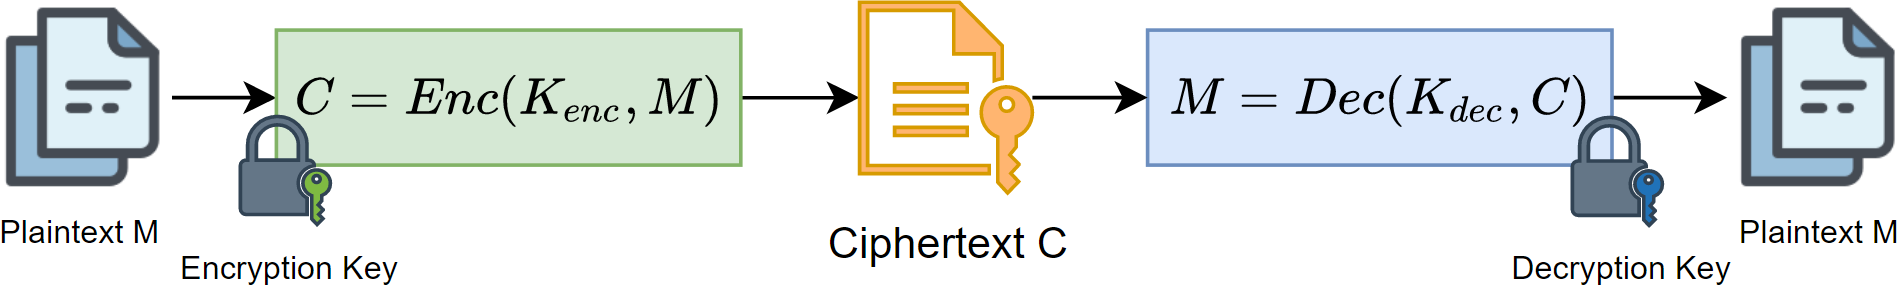
\includegraphics{image/asimmcrypto.png}
    \caption{Asymmetric Encryption Base Scheme}
    \label{fig:asymmcrypto}
\end{figure}\\
C'è un \textbf{importante MA:} gli algoritmi a chiave asimmetrica sono \textbf{computazionalmente onerosi} e non sarebbero praticabili per l'\textbf{intera} sessione di comunicazione cifrata.\\
C'è bisogno di un approccio \textbf{ibrido}:
\begin{itemize}
    \item Algoritmi Asimmetrici per \textbf{inizializzare} la comunicazione \textbf{sicura}
    \item Algoritmi Simmetrici per il \textbf{trasferimento sicuro} di informazioni.
\end{itemize}
\begin{definition}[Hybrid Approach for Persistent Communication]
\begin{enumerate}
    \item \textbf{Handshake/Session Key Exchange:} Viene utilizzata la \textbf{criptazione asimmetrica} per \textbf{scambiarsi informazioni} sulla \textbf{crittografia simmetrica} da utilizzare successivamente e \textbf{impostare} dei \textbf{segreti comuni (Key Agreement)} tra le due parti.\\
    \begin{remark}
    Dai segreti comuni vengono derivate le chiavi simmetriche, dette \textbf{Chiavi di Sessione}, usate nella\textbf{ criptazione simmetrica} e nel \textbf{controllo di integrità}.
    \end{remark}
    \item \textbf{Data Transfer:} le due parti \textbf{comunicano} in maniera sicura tra loro, tramite \textbf{meccanismi a chiave simmetrica}.
    \item \textbf{Rekeying:} eventualmente vengono \textbf{derivate nuove chiavi simmetriche} dagli \textbf{stessi} segreti comuni impostati precedentemente.
\end{enumerate}
\end{definition}
\section{Public Key Encryption \& Digital Signature}
Gli algoritmi asimmetrici utilizzano la \textbf{chiave} che viene condivisa, ovvero resa \textbf{pubblica}, durante la trasmissione dei dati. Poiché le chiavi pubbliche e private sono legate, vale la seguente proprietà:
\begin{proposition}[Pubkey Encryption]
In uno schema di cifratura con chiave pubblica e chiave privata, \textbf{chiunque} può cifrare un messaggio M, ma \textbf{soltanto} il \textbf{vero destinatario} può decifrarlo.
\end{proposition}
La firma digitale è un concetto ben diverso, che sfrutta l'ipotesi che le funzioni di $Enc$ e $Dec$ siano commutative e quindi:
\begin{equation}\label{eq:commut}
    Dec(Enc(M)) = Enc(Dec(M))
\end{equation}
Questo implica che, in un sistema a \textbf{firma digitale}, abbiamo la seguente proprietà:
\begin{proposition}[Digital Signature]
Il meccanismo di firma digitale \textbf{fornisce} sia\textbf{ message integrity} che l’\textbf{autenticazione della sorgente/mittente} (non repudiant). Viene \textbf{realizzato} utilizzando una \textbf{funzione hash crittografica H}, un \textbf{algoritmo di criptazione asimmetrico} e le \textbf{chiavi privata e pubblica del mittent}e, per generare una firma del messaggio. In particolare:
\begin{itemize}
    \item Il \textbf{mittente} genera la sua firma $sign_M=Dec_{src}(H(M))$, \textbf{criptando} la sua \textbf{chiave privata} il digest del messaggio M. Invia quindi \{M, $sign_M$\} al destinatario.
    \item Il \textbf{destinatario} legge la firma e \textbf{ottiene} il \textbf{digest} \textbf{decriptando} con la \textbf{chiave pubblica} del \textbf{mittente}.
    \[H(M)=Enc_{dest}(sign_M)\]
    Ricalcola quindi il digest dal messaggio ricevuto e lo confronta con quello ottenuto dalla firma.
    \item \textbf{Se i due digest corrispondono}, il \textbf{messaggio} è \textbf{integro} e \textbf{proviene con certezza dal mittente}.
\end{itemize}
\end{proposition}
\begin{note}
La funzione \textbf{hash} viene utilizzata\textbf{ senza chiave simmetrica} in quanto \textbf{ha} il solo \textbf{scopo} di \textbf{ridurre la dimensione dell’oggetto da criptare asimmetricamente}, così da rendere il meccanismo efficiente.\\
Inoltre, il \textbf{destinatario}, ovvero colui che ha necessità di verificare l’integrità del messaggio, \textbf{ha bisogno solamente della chiave pubblica del mittente}, ovvero di nessun segreto condiviso, a differenza del MAC che richiede una chiave simmetrica, ovvero un segreto noto a entrambe le parti.
\end{note}
\begin{figure}[h]
    \centering
    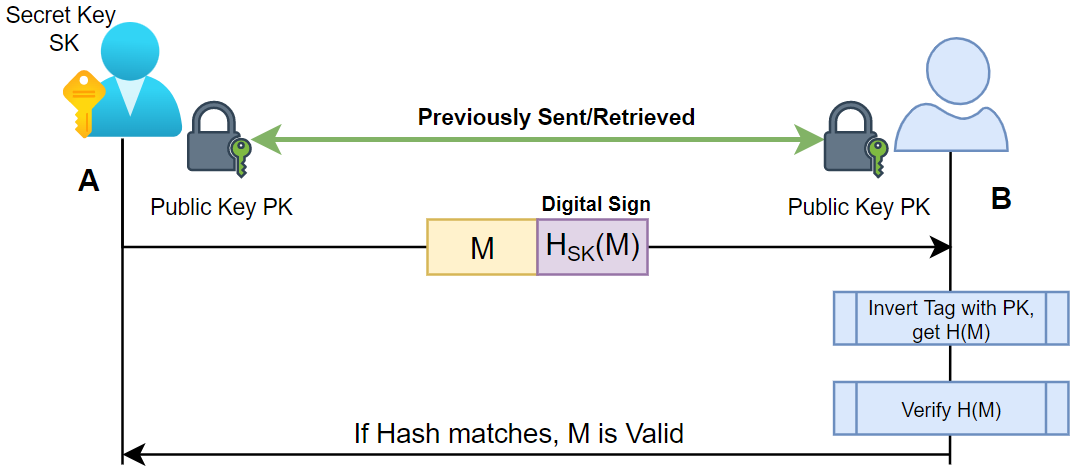
\includegraphics{image/digitalsign.png}
    \caption{Simple digital sign scheme}
    \label{fig:digitalsign}
\end{figure}
La firma digitale permette di avere un sistema più sicuro rispetto ad un semplice tag, in quanto siamo \textbf{certi} che chi ha firmato il documento è il vero autore. Difatti, in crittografia simmetrica, non è possibile dedurre l'autore del messaggio a partire dal tag, perché chiunque potrebbe produrlo. Nel caso della digital signature, vale invece la seguente proprietà
\begin{definition} [Non-Repudiation Property]
E' un concetto di sicurezza dove viene garantita l'integrità del messaggio che viene trasmesso, fornendo un identificatore per l'autore della firma.
\end{definition}

\section{Key Agreement Algorithms}
Il problema fondamentale di un meccanismo a chiave asimmetrica è che è necessario sviluppare un modo per condividere le chiavi ed instaurare il processo di \textit{Key Agreement}, ovvero un punto nel protocollo nel quale vengono fissate le chiavi da usare per scambiare i messaggi.\\
Supponiamo di suddividere la chiave $K$ in due parti $k_1,k_2$, allora il problema di ricostruire la chiave è facile se le due parti sono note, ma è difficile data la chiave capire quali sono le parti che la costituiscono. Gli algoritmi principali di key agreement sono due: RSA e Diffie-Hellman.\\
Un attaccante che vuole trovare la chiave in un sistema che usa questi algoritmi è di fronte a due problemi:
\begin{proposition}[Discrete Logarithm Problem in Prime Field]\label{prop:disclog}
Dati tre \textbf{numeri primi \textsc{GRANDI}} $p,g,x$ \textbf{è facile calcolare}; $y=g^x\mod{p}$.\\
Dato $y=g^x\mod{p}$ \textbf{è difficile calcolare}: $x=\log_g(y)\mod{p}$
\end{proposition}
\begin{proposition}[Product Factorization of Two \textbf{Large} Prime Numbers]\label{prop:prodfact}
Dati due \textbf{numeri primi \textsc{GRANDI}} $p,q$ \textbf{è facile calcolare}: $N=p\cdot{q}$.\\
Dato $N$ è \textbf{difficile trovare} la fattorizzazione in numeri primi di $p$ e $q$.
\end{proposition}
\begin{remark}
Per \textbf{"facile/difficile"} intendiamo che esiste o meno un algoritmo per il calcolo \textbf{efficiente} di quel valore.
\end{remark}
Vediamo perché calcolare $g^x$ è facile: 
\begin{algorithm}
\caption{Square and Multiply}\label{alg:squaremult}
\begin{algorithmic}[1]
\Procedure{exp\_by\_squaring}{$g,x$}\Comment{Fast compute $g^x$}
\If {$x=0$} 
    \Return 1
\ElsIf {$x=1$} 
    \Return g
\Else
\State $exp\gets x_2[1:]$\Comment{Take exponential in base 2 and cut the msb}
\State $r\gets g$
\ForAll{$b$ \textbf{in} $exp$}\Comment{Loop from $2_{\text{nd}}$ msb to the lsb of $exp$}
    \State $r\gets r^2$\Comment{For every bit, square $g$}
    \If {$b[i]==1$}\Comment{If current bit is 1, multiply by $g$}
       \State $r\gets r\times g$
    \EndIf  
\EndFor
\EndIf
\EndProcedure
\end{algorithmic}
\end{algorithm}\\
La complessità dell'algoritmo è ovviamente $O(log_2(x))=O(n)$ per i quadrati e $O(log_2(x)/2)=O(n/2)$ per le moltiplicazioni, con $n$ numero di bit necessari a costruire l'esponente.\\
L'algoritmo rappresenta un metodo veloce per calcolare un qualsiasi esponenziale, ma lavorando con il modulo, abbiamo una sovrapposizione notevole di valori per il quale rende difficile il problema del calcolo inverso.\\
Vediamo un esempio grafico del perché è difficile calcolare l'inversa di un esponenziale in modulo, graficando i punti di $y=3^x\mod104729$, con $x\in\{0,3000\}$\\
Vediamo i due principali algoritmi di key-agreement.
\begin{figure}[ht]
    \centering
    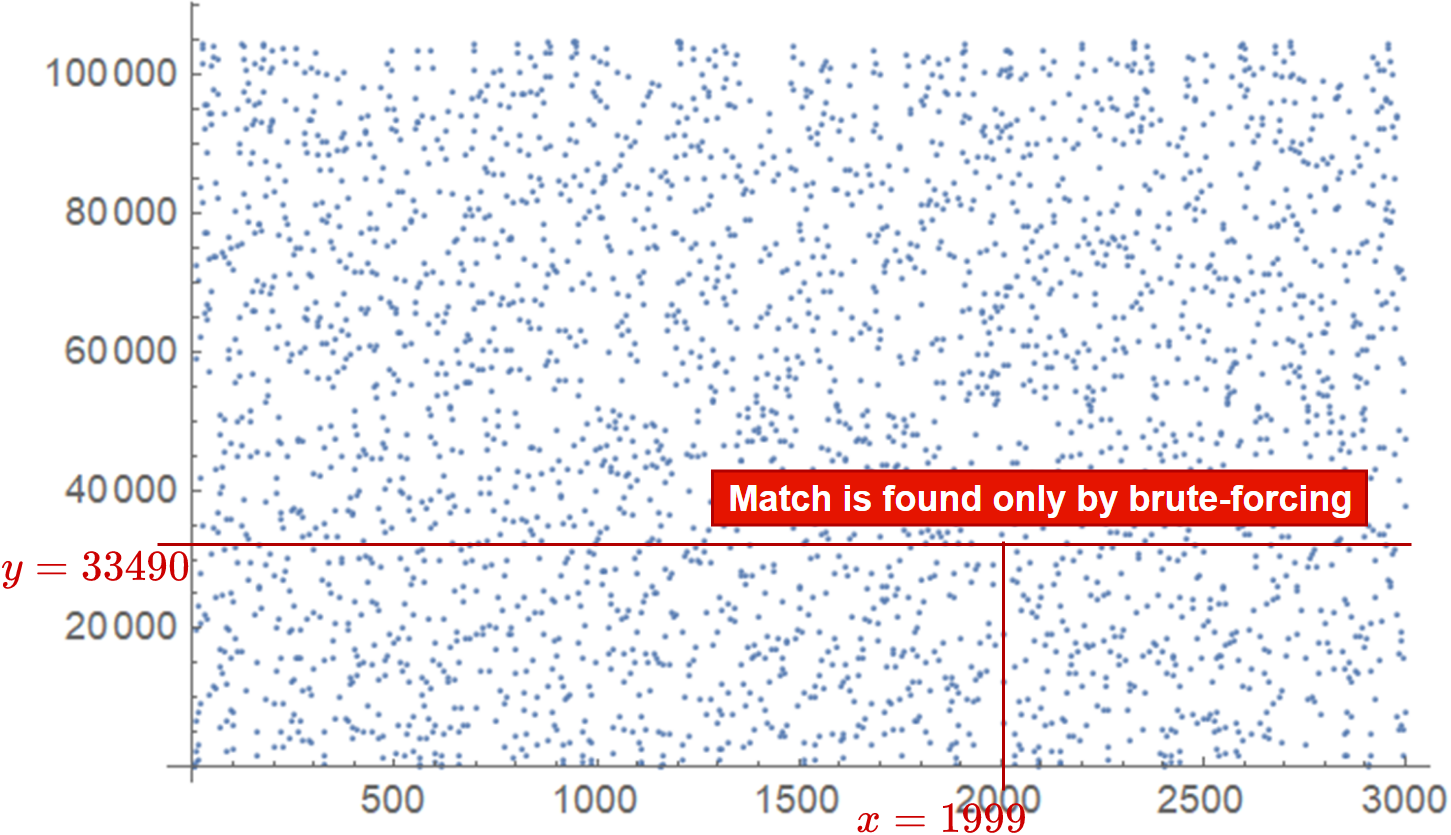
\includegraphics[width=0.7\textwidth]{image/descretelog.png}
    \caption{Descrete Logarithm Problem: How to invert the exponetial?}
    \label{fig:descretelog}
\end{figure}
\section{Diffie Hellman}
Lo scopo dell'algoritmo è \textbf{esclusivamente} lo scambio di chiavi. L'idea si basa sul calcolo dell'esponenziale in modulo dei numeri primi. Questo permette di rendere arduo il calcolo inverso. L'algoritmo lavora al seguente modo:\pagebreak
\begin{definition}[(Vanilla) Diffie-Hellman]\label{def:dh}
Consideriamo due utenti A, che \textbf{genera un rnd} $x$, B che \textbf{genera un rnd} $y$. \textbf{Queste sono le chiavi private degli utenti}.\\
Assumiamo che vengano precedentemente scambiati i parametri $g,p$\footnote{In realtà $p$ deve avere delle proprietà particolare che vedremo poi}, rispettivamente \textbf{base} dell'esponenziale e \textbf{numero primo GRANDE}.
\begin{enumerate}
    \item A invia $g^x\mod{p}$
    \item B invia $g^x\mod{p}$
    \item A calcola $K=(g^y)^x\mod{p}$
    \item B calcola $K=(g^x)^y\mod{p}$
\end{enumerate}
Adesso i due utenti hanno le chiavi necessarie.
\end{definition}
\begin{remark}Nonostante è vero che un attaccante che intercetta i due messaggi non può calcolare $g^{xy}$ con facilità, vedremo che non bisogna \textbf{MAI} usare Diffie-Hellman così come è fatto in quanto un MITM è dietro l'angolo. 
\end{remark}
\begin{note}
DH \textbf{NON SUPPORTA} la firma digitale e lo scambio di messaggi.
\end{note}
\subsection{Implementazioni di DH}
L'algoritmo di Key Agreement di DH è stato implementato in tre modi. Nella sua versione \textit{\textbf{Vanilla}} viene detto anche \textbf{Anonymous DH}, perché i valori $x$ e $y$ sono \textbf{generati dinamicamente} ma \textbf{non autenticati}. Tuttavia questo metodo risulta poco sicuro a fronte di attacchi MITM come possiamo vedere in \cref{fig:mitmdh}
\begin{figure}[ht]
    \centering
    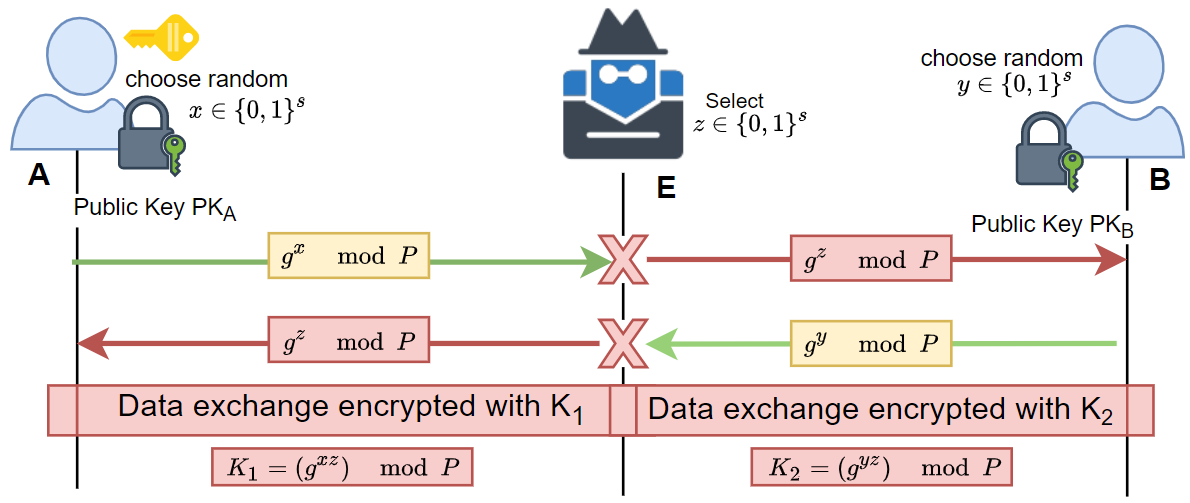
\includegraphics{image/mitmdh.png}
    \caption{MITM in DH Key Agreement}
    \label{fig:mitmdh}
\end{figure}\\
Se i messaggi fossero stati autenticati tramite firma, questo non sarebbe successo.
Per sopperire a questa vulnerabilità abbiamo due implementazioni aggiuntive: 
\begin{definition}[Fixed DH]\label{def:fixdh}
A genera un numero $x$, B un numero $y$. Vengono allora calcolati rispettivamente $g^x\mod(P)$ e $g^y\mod(P)$.\\
I due coefficienti pubblici vengono \textbf{mantenuti statici} e \textbf{firmate} da una Certification Authority (\cref{def:ca}). A questo punto si procede con il key agreement in versione standard.
\end{definition}
\begin{corollary}[Vulnerabilites of Fixed DH]
Il segreto $g^{xy}\mod(P)$ è ora sempre lo stesso e hardcoded nel certificato, pertanto andrà \textbf{sempre usato quello} per le future connessioni fino alla sua scadenza (\cref{sssec:digitalcert}). Questo genera problemi nel caso di attacchi particolari, che sfruttano una mole di dati che si estende per un lasso temporale molto ampio (anche anni).\\
\textbf{Conseguenza:} Esposizione a \textbf{dictionary attacks}.
\end{corollary}
\begin{definition}[Ephimeral DH]\label{def:ephdh}
A genera un numero $x$, B un numero $y$. Vengono allora calcolati rispettivamente $g^x\mod(P)$ e $g^y\mod(P)$ e auto-firmati da loro stessi.
Durante il processo di scambio insieme ai coefficienti pubblici vengono inviati anche i rispettivi certificati, firmati da una CA. Vengono scambiati quindi i seguenti pacchetti:
\begin{table}[H]
    \centering
    \begin{tabular}{c c}
         \textbf{A invia}& \textbf{B invia} \\
        $(A, g^x)_{A\_sign}$ & $(A, g^y)_{B\_sign}$ \\
         $(A, PK_A)_{CA\_sign}$&$(B, PK_B)_{CA\_sign}$
    \end{tabular}
\end{table}
\begin{remark}
Questa variante permette di cambiare il coefficiente pubblico a piacere, in quanto l'identità delle entità coinvolte sarà certificata dalla CA
\end{remark}
\end{definition}
\begin{corollary}[Vulnerabilities of Ephimeral DH]
Gli \textbf{attacchi MITM} sono \textbf{bloccati} dal fatto che i \textbf{coefficienti pubblici} sono \textbf{firmati da una CA} e il coefficiente può essere generato localmente quante volte si vuole. 
\end{corollary}
\section{RSA}
Algoritmo sviluppato da \textit{Rivest, Shamir, Adleman} nel '77 e brevettato fino al 2000, RSA è tra gli algoritmi di cifratura più famosi al mondo. Si basa sul problema della fattorizzazione di numeri primi (\cref{prop:prodfact}) e sulla \textbf{modular exponentiation} per cifrare e decifrare i messaggi.
\begin{proposition}[RSA Encryption]\label{prop:rsaenc}
Dato un messaggio $m$, una \textbf{chiave pubblica} $K_{pub}$ e un numero primo \textbf{grande} $N$
\begin{equation}
    C = (m)^{K_{pub}}\mod{N}
\end{equation}
\end{proposition}
\begin{proposition}[RSA Encryption]\label{prop:rsadec}
Dato un messaggio cifrato $C$, una \textbf{chiave privata} $K_{sec}$ e un numero primo \textbf{grande} $N$
\begin{equation}
    m = (C)^{K_{sec}}\mod{N}
\end{equation}
\end{proposition}
Vediamo però un esempio:
\begin{example}
Poiché per costruzione l'algebra modulare comporta l'introduzione di un \textbf{periodo} lungo quanto il numero rispetto cui viene calcolato, $m^x\mod{N}$ è periodica e abbiamo un problema di \textbf{ciclicità}.
\begin{equation*}
    \begin{aligned}
    3^x\mod{10}&={\textcolor{red}{3,9,7,1},3,9,7,1,\dots}\\
    7^x\mod{10}&={\textcolor{red}{7,9,3,1},7,9,3,1,\dots}\\
    9^x\mod{10}&={\textcolor{red}{9,1},9,1,9,1,\dots}\\
    \end{aligned}
\end{equation*}
\end{example}
\begin{remark}
RSA supporta sia firma digitale che la cifratura.
\end{remark}
Il teorema di \textit{Eulero-Fermat} permette di calcolare il \textbf{periodo} dell'esponente modulare:
\begin{proposition}[Euler's Totient Function]
Sia $\Phi(N)=E$ il massimo periodo. Se $m,N$ sono coprimi ($GCD(m,N)=1$), allora
\begin{equation}\label{eq:eulertot}
    m^{\Phi(N)}\mod{N}=1 
\end{equation}
\end{proposition}
Calcoliamo la funzione \cref{eq:eulertot} nel caso di RSA. 
\begin{itemize}
    \item Sia $p$ un numero primo, allora $\Phi(p)=p-1$ per costruzione.
    \item Siano $p,q$ primi. Allora \[\Phi(p\cdot{q})=\Phi(p)\cdot\Phi(q)=(p-1)(q-1)\]
    \item Sia $p^k$ un numero primo, allora 
    \[\Phi(p^k)=\Phi(p)\cdot p^{k-1}=(p-1)\cdot p^{k-1}\]
    \item Generalmente, se $N=\prod_{i=1}^{z}p_i^{k_i}$, allora
    \[\Phi(N)=\prod_{i=1}^{z}(p_i-1)p_i^{k_i-1}\]
\end{itemize}
Il caso di RSA è ovviamente $Phi(p\cdot{q})$. La conseguenza della periodicità in RSA è dimostrabile con un esempio:
\begin{example}
Consideriamo $2^x\mod{11}=\{2,4,8,5,10,9,7,3,6,1\}$. Poiché $p=11$ è primo, allora $Phi(11)=10$. Supponiamo di calcolare $9\cdot7\mod11$.
\begin{itemize}
    \item \textbf{Moltiplicazioni mod11:} $9\cdot7\mod11=63\mod11=8$
    \item \textbf{Approccio alternativo:} Osserviamo che $9=2^6\mod11$ mentre $7=2^7\mod11$. Allora:
    \[9\cdot7\mod11=2^6\cdot2^7\mod11=2^{13}\mod11=2^{10+3}\mod11=1\cdot2^3\mod11=8\]
\end{itemize}
\begin{note}
La conseguenza quindi è che se dobbiamo calcolare l'esponente ad una potenza elevata qualsiasi, possiamo calcolare direttamente $g^{x\mod\Phi(N)}\mod N$, invece di calcolare il vero esponente.
\end{note}
\end{example}\pagebreak
\subsection{RSA Key Transport}
Vediamo ora come  l'algoritmo costruisce le sue chiavi.
\begin{definition}[RSA Key Generation]\label{def:rsakey}
\begin{enumerate}
    \item Generare due numeri primi \textbf{grandi}: $p,q$ che \textbf{devono restare segreti}
    \item Calcolare l'\textbf{RSA module:} $N=p\cdot q$. Questo \textbf{numero} è reso \textbf{pubblico}.
    \item Calcolare $\Phi(N)=(p-1)(q-1)$, che \textbf{deve restare segreto}.
    \item \textbf{Generare una chiave pubblica} $e$ che sia \textbf{coprima con $\Phi(N)$}. Ovvero: 
    \[1<e<\Phi(N)\]
    \item \textbf{Generare una chiave privata} $d$ tale che
    \[e\cdot d=1\mod\Phi(N)\]
    \[d=e^{-1}\mod\Phi(N)\]
\end{enumerate}
\begin{remark}
Generare una private-key in questo modo è possibile \textbf{se solo se} $e$ è invertibile in $\mod(\Phi(N))$, per questo serve che siano \textbf{coprimi}. Se $\Phi(N)$ \textbf{è segreto}, è ovviamente difficile calcolare $d$ partendo da $e$.
\end{remark}
\end{definition}
Vediamo l'effetto di questa generazione delle chiavi:
\[C=M^e\mod N\]
\[M=C^d\mod N=(M^e)^d\mod N=M^{ed}\mod N=M^1\mod N = M\]
\begin{definition}[Algoritmo di Euclide Esteso]\label{def:exteuclid}
Consideriamo l'\textbf{identità di Bézout}: Dati due interi $a,b$, allora $\exists x,y$ coefficienti tale che
\[ax+by=MCD(a,b)\]
Per trovare $x,y$, costruiamo la seguente tabella:
\begin{center}
\begin{tabular}{|c|c|c|c|}
\hline
    x & y & r & q \\
\hline
    $1$ & $0$ & $\max\{a,b\}$& - \\ 
\hline
    $0$ & $1$ & $\min\{a,b\}$& $a/b$\\
 \hline
    \dots&\dots&\dots&\dots\\
\hline
    $x_{i-2}-r_{i-1}\cdot{x_{i-1}}$&$y_{i-2}-r_{i-1}\cdot{y_{i-1}}$&
    $rest(q_{i-2}/q_{i-1})$&$q_{i-2}/q_{i-1}$\\
\hline
    \dots&\dots&\dots&\dots\\
\hline
    $x^*$&$y^*$&$1$&-\\
\hline
\end{tabular}
\end{center}
I coefficienti cercati sono nell'ultima riga della tabella, che conterrà tante righe quante sono necessarie a far apparire $1$ nella colonna delle $q$. 
\end{definition}
\begin{example}[ Why RSA works?]
Supponiamo di essere in uno scenario di \textit{Decryption Challenge}: Dati $N,e$ e il messaggio cifrato $m^e$, calcolare la chiave di decifrazione (quella privata) $x$ tale che \[(m^e)^x\mod(N)=m\]
Normalmente sarebbe un problema difficile risolvere il problema perché l'unico modo è fare brute force sui possibili valori di $x$. \textbf{Se conosciamo} $\Phi(N)$ allora in tempo polinomiale è possibile trovare la soluzione della seguente equazione:
\[x=e^{-1}\mod\Phi(N)\]
\end{example}
\begin{example}[ Compute RSA Inverse]
Consideriamo uno scenario dove $e=K_{pub}=13$ e $N=77=11\times7$. Allora $\Phi(77)=10\times6=60$. Osserviamo che $MCD(e,\Phi)=1$ e quindi sono coprimi. Vogliamo calcolare la chiave privata $d$.\\
Innanzitutto calcoliamo i coefficienti $a,b$ tali che $\Phi a+eb=1$
\begin{center}
\begin{tabular}{|c|c|c|c|}
\hline
    x & y & r & q \\
\hline
    $1$ & $0$ & $60$& - \\ 
\hline
    $0$ & $1$ & $13$& $4$\\
 \hline
    $1$ & $-4$ & $8$ & $1$  \\
\hline
    $-1$ & $5$ & $5$ & $1$\\
\hline
    $-2$ & $-9$ & $3$ & $1$\\
\hline
    $-3$ & $14$& $2$&$1$\\
\hline
    $5$ & $-23$ & $1$ & -\\
\hline
\end{tabular}
\end{center}
Allora: $60\times5+13\times(-23)=1$. Per cui: $13^{-1}\mod60=-23$ e quindi $d=60-23=37$.
\end{example}
\begin{example}[ RSA toy example]
Supponiamo di applicare RSA, con $p=11,q=17,N=11\times17=187$. Abbiamo quindi la fattorizzazione in numeri primi e il numero su cui calcolare il modulo. Allora:
\[\Phi=(p-1)\times(q-1)=10\times16=160\]
Scegliamo la chiave pubblica nell'intervallo $\{1,160\}$: $e=7$. Allora:
\[d=7^{-1}\mod160=23\]
\begin{remark}
$23\times7\equiv=161=160+1=1\mod160$
\end{remark}
Abbiamo allora:
\begin{center}
    \begin{tabular}{c c}
     Enc: & $C=M^7\mod187$ \\
     Dec: & $M=(M^7)^{23}\mod187=M^{7\times23}\mod187=M$ \\
     Digital Sign: & $TAG=H(M^{23})\mod187$\\
     Verify Sign: & $H(M)=(TAG)^7\mod187=(H(M^{23}))^7\mod187$
\end{tabular}
\end{center}
Per verificare l'integrità, basta controllare che l'hash calcolato su M sia quello dedotto dalla firma.
\end{example}
\subsection{Bleichenbacher's Oracle}
\begin{definition}[Non-Malleability]
Diremo che un protocollo \textbf{non è malleabile} se, dato un messaggio cifrato $C$ di un plaintext $M$, un attaccante \textbf{NON} è in grado di creare un ciphertext differente $C'$ la cui decriptazione porta ad un messaggio $M'$ che è \textbf{in qualche modo legato} ad $M$
\end{definition}
RSA presenta un problema fondamentale, è \textbf{malleabile}. 
il protocollo di key-transport di RSA (\cref{def:rsakey}) è vulnerabile al Bleichenbacher Oracle, ovvero un attacco \textbf{Adaptive CCA}, che sfrutta la costruzione del padding in RSA, la sua \textbf{\textit{malleabilità}} ed eventuali messaggi di error signaling della \textit{specifica implementazione} del protocollo, al fine di \textbf{ricostruire il plaintext}.
\begin{definition}[Bleichenbacher's Oracle]\label{def:bleichenoracle}
Supponiamo che l'implementazione di RSA fornisca un modo per \textbf{determinare il primo bit del plaintext} $M$, generato dalla \textbf{decriptazione} all'arrivo di un \textbf{ciphertext arbitrario}\footnotemark.\\
\footnotetext{\textsuperscript{\thefootnote}Stiamo chiedendo che esista un \textbf{oracolo} di \textbf{decrittazione} solamente per il primo bit.}
L'attaccante pyuò effettuare il seguente \textbf{CCA}:
\begin{enumerate}
    \item Sia $C=M^e\mod(N)$ il \textbf{ciphertext obiettivo}.
    \item Sia $r=1$ e calcoliamo 
    \begin{equation*}
        \begin{aligned}
            C'&=((C\mod(N))\cdot(r^e\mod(N)))\mod(N)=\\
            &=(C\cdot r^e)\mod(N)\equiv(M\cdot r)^e\mod(N)
        \end{aligned}
    \end{equation*}
    \item \textbf{Inviamo} al sistema $C'$ per farlo \textbf{decifrare}. Per l'assunzione iniziale \textbf{otteniamo} il \textbf{primo bit} di ($M\cdot r$).\footnotemark
    \footnotetext{\textsuperscript{\thefootnote}In particolare il primo bit di $M$ coincide con quello di $M\cdot r$ se shiftato a sinistra di $log_2(\#bits_r)$}
    \item Moltiplicando per $r^{-1}$ troviamo il bit di $M$. 
    \item Ponendo $r=r\cdot2$ possiamo ripetere il processo e scoprire tutto $M$
\end{enumerate}
\end{definition}
\begin{note}
Con un bleichenbacher oracle servono al più $log_2(n)$ tentativi per decifrare $M$. con $n=log_2(M)$bits
\end{note}
\section{Pub-Key Infrastructure}
Consideriamo uno scenario di key agreement (scambio di chiavi pubbliche e setup di chiavi private comuni per creare un canale sicuro). Fino ad ora non ci siamo preoccupati di verificare la validità della chiave pubblica rilasciata da un utente e l'abbiamo solo usata per decifrare il tag aggiunto al messaggio per ottenere l'hash di $M$ nel caso della firma digitale, oppure per stabilire una chiave comune per la cifratura del canale di comunicazione con RSA. 
\begin{figure}[ht]
    \centering
    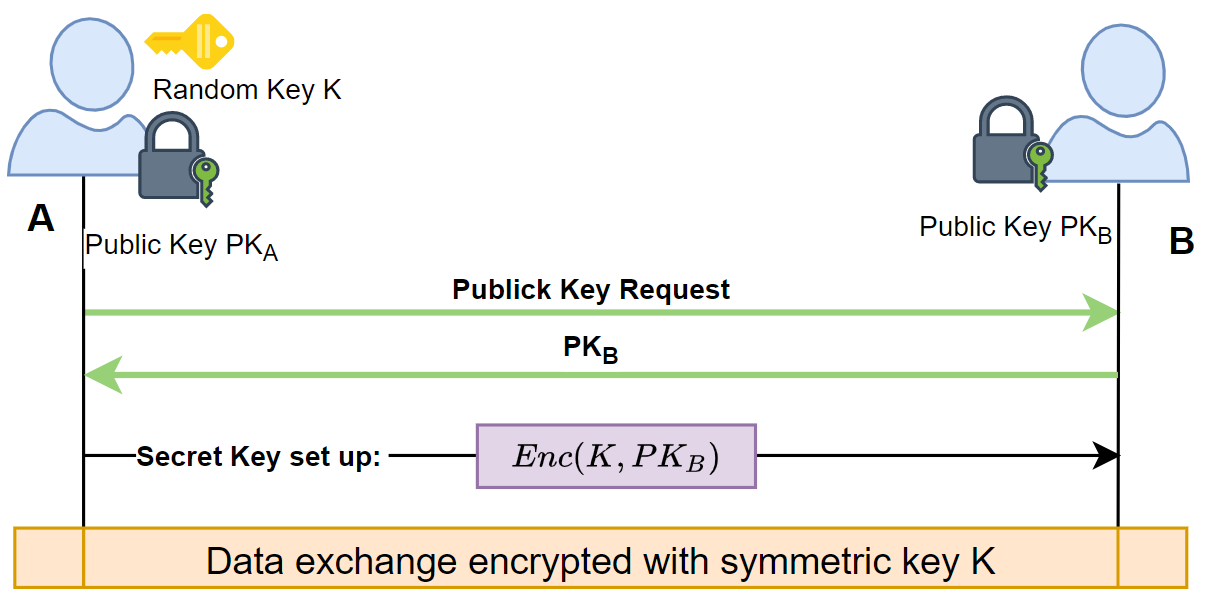
\includegraphics[width=\textwidth]{image/rsakeytrans.png}
    \caption{RSA Key Transport}
    \label{fig:rsakeytrans}
\end{figure}
\begin{note}Se un attaccante rispondesse alla richiesta di un utente di scaricare una chiave pubblica e la sostituisse con la propria, allora ogni messaggio inviato da quel momento in poi dall'attaccante sarebbe considerato valido perché la public key è stata sostituita. 
\end{note}
Vediamo lo schema di un possibile attacco ad RSA:
\begin{figure}[ht]
    \centering
    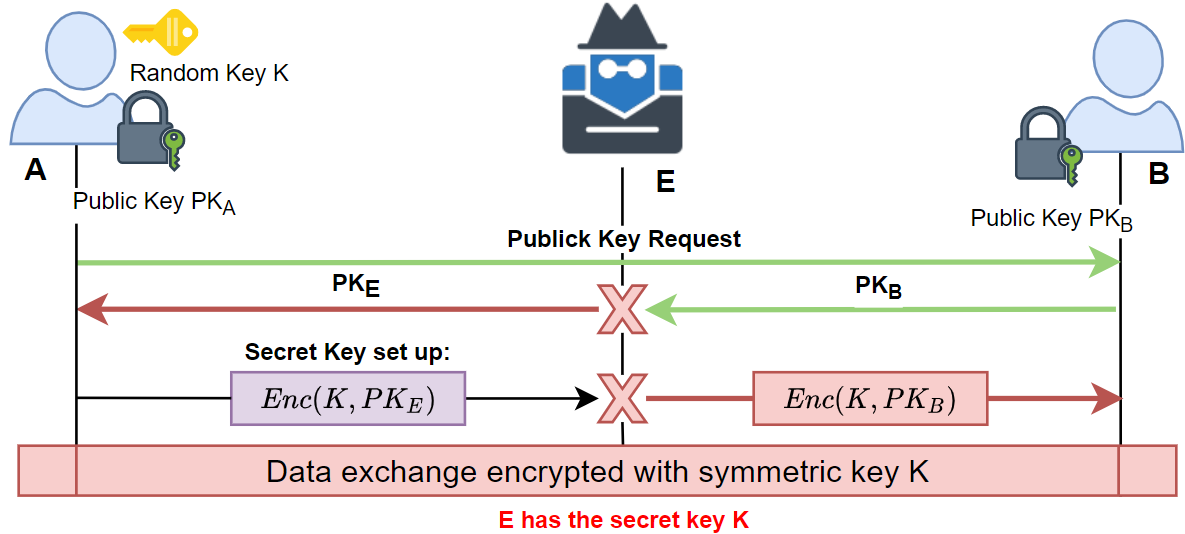
\includegraphics{image/mitmrsa.png}
    \caption{MITM in RSA Key Transport}
    \label{fig:mitmrsa}
\end{figure}\\
\begin{remark}
Diffie-Hellman non avrebbe comunque protetto da questo tipo di MITM, vedi \cref{fig:mitmdh}
\end{remark}
\begin{proposition}
Per scambiare le chiavi \textbf{è necessario} legare in \textbf{modo crittografico} la \textbf{chiave pubblica} all'\textbf{identità}.
\end{proposition}
Abbiamo bisogno di un'infrastruttura che, oltre a definire lo scambio di chiavi, definisca \textbf{protocolli}, \textbf{strategie} e \textbf{meccanismi} affinché \textbf{lo scambio sia sicuro}\pagebreak
\subsection{Digital Certificate}\label{sssec:digitalcert}
Un modo per essere sicuri della chiave pubblica rilasciata da un utente è quella di \textbf{fidarsi di un'entità terza}, detta \textbf{Certification Authority}, che garantisce l'integrità del legame che c'è tra la chiave e l'identità.
\begin{definition}[Certification Authority]\label{def:ca}
Una CA è una \textbf{Trusted Third Party} a cui altre entità si affidano per ricevere dei certificati di affidabilità.
\end{definition}
\begin{remark}
Una soluzione più semplice sarebbe quella di fare in modo che tutti conoscano le chiavi pubbliche degli utenti con i quali si vuole comunicare, ma questa soluzione \textbf{non è} ovviamente \textbf{scalabile}.
\end{remark}
\begin{note}
I certificati digitali non risolvono il problema, perché potrebbe esserci un modo di falsificarli.
\end{note}
Il modo con cui una CA rilascia un certificato è il seguente:
\begin{proposition}[Emissione di un Certificato]
Un'entità verifica \textbf{(e.g. offline)}, presso una CA, la sua identità. Vengono svolte le seguenti operazioni:
\begin{enumerate}
    \item L'entità genera una $PK$ e una $S_K$, che viene \textbf{mantenuta segreta}.
    \item L'entità comunica la sua $PK$ alla CA tramite un \textbf{canale sicuro}
    \item La CA fa le verifiche del caso e se passano tutte emette un \textbf{certificato firmato}:
    \[cert=(name_{entity}, PK)_{CA\_sign}\]
\end{enumerate}
\end{proposition}
Il modo con cui un utente si accerta che un certificato è autentico è il seguente:
\begin{definition}[Verifica della Validità di un Certificato]\label{def:certval}
Un'entità $A$ vuole accertarsi che il \textbf{certificato} di $B$ sia corretto e di \textbf{sua proprietà}. Vengono svolte le seguenti operazioni:
\begin{enumerate}
    \item A contatta B e ne \textbf{richiede} il \textbf{certificato}.
    \item B invia ad A la tripla: $\{name_B, PK_B, CERT_B\}$, dove \[CERT_B=(name_B. PK_B)_{CA\_sign}\]
    \item A verifica che $CERT_B$ sia stato emesso da una \textbf{CA fidata} per lui e che la \textbf{firma sul certificato} sia corretta.
    \item A si accerta dell'\textbf{identità} di B con una procedura "\textbf{chap-like}" (\cref{fig:chap}) in uno dei modi seguenti:
    \begin{itemize}
        \item \begin{enumerate}
        \item A invia una nonce a B
        \item B risponde ad A \textbf{firmando} la \textbf{nonce} con la \textbf{sua chiave segreta} $SK_B$.
    \end{enumerate}
    \item \begin{enumerate}
        \item A invia una challenge contenente una cifratura a B
        \[Chall=Enc(nonce)_{PK_B}\]
        \item B risponde ad A con la nonce ottenuta decifrando la challenge con la sua $SK_B$ 
        \[nonce = Dec(Chall)_{SK_B}\]
    \end{enumerate}
    \end{itemize}
\end{enumerate}
\end{definition}
\begin{note}
Il metodo chap-like per verificare l'identità dell'entità con cui vogliamo collegarci è \textbf{necessario} per evitare replay attack sul certificato.
\end{note}
Le CA sono molte e dislocate in tutto il mondo, organizzate poi in una struttura gerarchica. Un'architettura PKI definisce proprio queste relazioni e anche gli standard a cui i certificati devono aderire. Un esempio di certificato è il seguente:
\begin{example}[ Certificate X.509 (High Level View)]
\begin{multicols}{2}
\begin{itemize}
    \item \textbf{Versione Standard:} Indica la versione del certificato.
    \item \textbf{Validità Temporale:} Data di inizio e fine validità.
    \item \textbf{Numero Seriale:} Identificatore univoco del certificato.
    \item \textbf{Algoritmi:} Algoritmi crittografici supportati dal certificato. Detta anche \textbf{Cipher Suite}
    \item \textbf{Identità CA:} Nome della CA che ha emesso il certificato.
    \item \textbf{Identità Utente:} nome dell'utente associato al certificato.
    \item \textbf{Chiave Pubblica Utente:} chiave pubblica dell'utente.
    \item \textbf{Firma Digitale:} firma del certificato generata dalla CA.
\end{itemize}
\columnbreak
\begin{figure}[H]
    \centering
    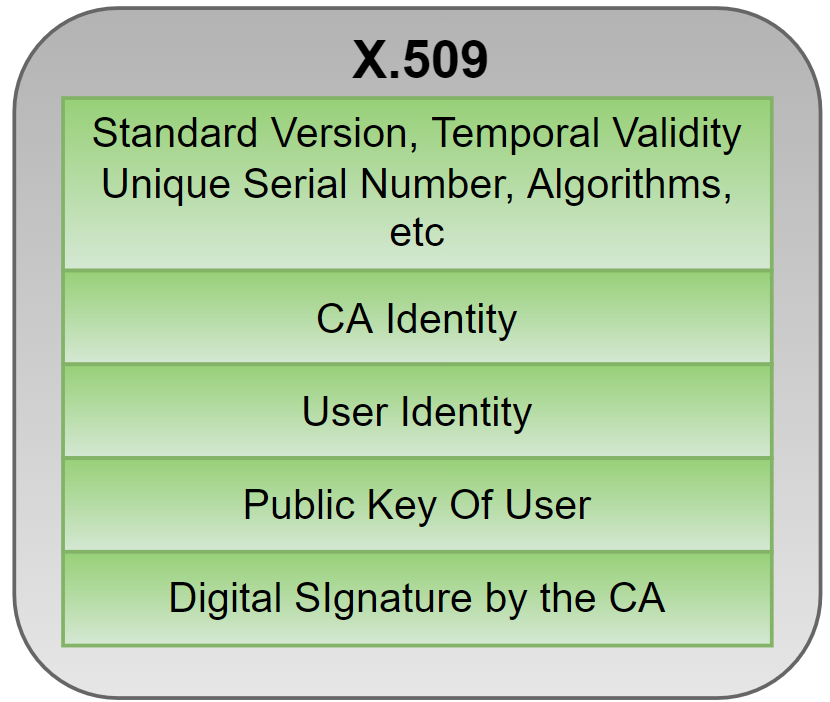
\includegraphics[width=0.48\textwidth]{image/x509.png}
    \caption{Certificate X.509}
    \label{fig:certx509}
    \vspace{-7pt}
\end{figure}
\begin{itemize}
    \item \textbf{Estensioni:} (se X.509v3) campo addizionale che può contenere diversi tipi di attributi e permette di espandere il certificato con nuove feature.
\end{itemize}
\end{multicols}
\end{example}
\subsection{Certificate Revocation List}
Ogni PKI \textit{\textbf{deve}} includere un meccanismo di \textit{revoca} dei certificati, poiché questi possono essere \textbf{compromessi}. Ad esempio: 
\begin{itemize}
    \item La chiave privata è stata persa o divulgata.
    \item La chiave pubblica è obsoleta e non più utilizzata.
    \item Il certificato è scaduto.
\end{itemize}
Esistono 2 approcci per la revoca di un certificato:
\begin{itemize}
    \item \textbf{Revocazione Implicita:} avviene se il \textbf{periodo di validità} di un certificato si esaurisce.
    \item \textbf{Revocazione Esplicita:} avviene quando effettuata per \textbf{\textit{Certificate Revocation List}}
\end{itemize}
\begin{definition}[Certificate Revocation List]
Una CRL è una lista mantenuta da \textbf{OGNI} CA, che periodicamente \textbf{deve} essere \textbf{aggiornata} con i certificati che la CA ha \textbf{rimosso}.\\
Possiede il seguente formato:
\begin{itemize}
    \item \textbf{Emittente (Issuer):} Indica la CA che ha \textbf{pubblicato} la lista.
    \item \textbf{Ultima Data di Aggiornamento:} ultima data in cui la lista è stata modificata.
    \item \textbf{Prossima Data di Aggiornamento:} data futura in cui verrà pubblicato il prossimo aggiornametno. Indica il periodo di validità della lista.
    \item \textbf{Elenco dei Seriali Revocati:} indica i numeri seriali dei \textbf{certificati da revocare}.
    \item \textbf{Elenco della Data di Revocazione}.
    \item \textbf{Firma Digitale:} firma generata dalla CA emittente della lista.
\end{itemize}
\end{definition}
\begin{note}
Ogni entità che utilizza un certificato \textbf{dovrebbe sempre verificarne la validità} controllando la relativa CRL. Tuttavia, questa operazione è demandata ad applicazioni che svolgono un ruolo \textbf{critico} nella rete, per alleggerire il carico complessivo.
\end{note}
\subsection{Public Key Criptography Standards}
La PKI specifica molti aspetti legati alla \textbf{crittografica asimmetrica}. Gli standard sono definiti dalle:
\begin{definition}[PKCS]
Public Key Criptography Standards
\end{definition}
Attualmente vanno dal numero 1 al numero 15, alcuni di questi sono: 
\begin{itemize}
    \item \textbf{PKCS\#1:} RSA
    \item \textbf{PKCS\#3:} DH
    \item \textbf{PKCS\#6:} Estensione del formato \textbf{X.509}. Alcune delle estensioni più comuni sono:
    \begin{proposition}[X.509 Extensions]
    \begin{itemize}
        \item \textbf{Authority Key Identifier:} identifica la chiave pubblica corrispondente alla chiave privata \textbf{usata per firmare un certificato}.
        \item \textbf{Subject Key Identifier:} Identifica i certificati che contengono al loro interno una determinata chiave pubblica.
        \item \textbf{Key Usage:} Specifica lo scopo della chiave contenuta nel certificato. Ovvero, per quale meccanismo può essere utilizzata.
        \item \textbf{Subject Alternative Name:} permette di associare più identità al soggetto del certificato, che possono aggiungersi o rimpiazzare le precedenti.
        \item \textbf{Extended Key Usage:} Specifica ulteriori scopi per la chiave pubblica contenuta nel certificato. che ossono aggiungersi o rimpiazzare quello specificato nell'estensione precedente.
    \end{itemize}
    \end{proposition}
    \item \textbf{PKCS\#10:} \textbf{CRSS (Certification Request Syntax Standard)}. Specifica il formato dei messaggi di richiesta dei certificati. Un esempio è il seguente:
    \begin{proposition}[Certification Signing Request - CSR]
    Messaggio inviato da parte di una CA al fine di \textbf{applicarsi per un certificato} della \textbf{sua identità digitale}. Le operazioni svolte dall'applicante sono:
    \begin{enumerate}
        \item Genera una coppia di chiavi, pubblica e privata. L'ultima viene mantenuta segreta.
        \item Genera un \textbf{CSR}, contenente le informazioni per identificarsi: Nome, Chiave pubblica e, eventualmente, alcune estensioni.
        \item Il \textbf{CSR} viene \textbf{inviato} \textbf{insieme} ad \textbf{altre credenziali} o \textbf{prove di identità} richieste dalla CA. Inoltre, quest'ultima può contattare l'applicante per richiedere ulteriori informazioni.
    \end{enumerate}
    \end{proposition}
    \item \textbf{PKCS\#11:} \textbf{CTIS (Cryptographic Token Interface Standard)}. Specifica l'API per \textbf{firmare e verificare} dati da parte di un dispositivo che mantiene chiavi.
    \item \textbf{PKCS\#12:} \textbf{PIESS (Personal Information Exchange Syntax Standard)}. Specifica il \textbf{formato} dei file utilizzati per \textbf{memorizzzare i certificati} e le \textbf{chiavi private} usati per spostare informazioni riservate tra diversi browsers.
    \item \textbf{PKCS\#13:} \textbf{ECC (Elliptic Curve Cryptography)}
\end{itemize}
\subsection{Certificate Chains}
Per distribuire le responsabilità e il carico delle certificazioni digitali, le CA vengono \textbf{organizzate} secondo una \textbf{gerarchia ad albero} dove i nodi radice sono considerati, per definizione, i più sicuri.\\
L'ovvio problema di questa struttura gerarchica è che, eccezion fatta per la radice, \textbf{non abbiamo garanzie} che un particolare nodo dell'albero sia \textbf{trusted}, ovvero che a sua volta la sua identità sia verificata. Sono necessari dei meccanismi aggiuntivi, detti proprio \textbf{certificate chains}.\\
\begin{remark}
I meccanismi aggiuntivi sono \textbf{necessari} in quanto su una singola macchina non è possibile salvare tutti i certificati di tutto il mondo, serve qualcosa di scalabile, come un database distribuito.
\end{remark}
\begin{definition}[Certificate Chain]
Una catena è una lista di certificati seguiti da una o più CA, con le seguenti proprietà:
\begin{itemize}
    \item L'entità che rilascia il certificato è collegata alla prossima in lista. 
    \item \textbf{Ogni} certificato, a parte l'ultimo, è firmato dalla chiave segreta corrispondente al prossimo certificato nella catena.
    \item L'\textbf{ultimo} certificato in lista è un \textbf{trust anchor}, del quale l'utente si fida perché gli è stato fornito tramite una procedura attendibile. Dalle trust anchor inizia il processo di validazione.
\end{itemize}
\end{definition}
Una delle estensioni che è possibile trovare nel certificato è la seguente:
\begin{theorem}[Basic Constraint]\label{thm:basiccons}
E' un valore booleano, che indica se il l'entità legata a al certificato ha o meno il permesso di utilizzare la propria chiave privata per firmare altri certificati.
\end{theorem}
\begin{remark}
Permette di individuare un certificato illegittimo nella catena.
\end{remark}
\begin{note}
Una compagnia può avere un cosiddetto \textbf{Wildcard Certificate}. E' un certificato jolly, che permette di certificare tutti i suoi sistemi, con nome diverso, in uno stesso dominio.
\end{note}\pagebreak
Il meccanismo di certificazione è simile a quello espresso in \cref{def:certval}, ma questa volta c'è almeno un nodo intermedio in più.
\begin{definition}[Certificate Chain Procedure]\label{def:certchain}
Supponiamo che A voglia autenticare B. Supponiamo che \textbf{$CA_B$} sia la certificante di B e che $U$ sia la root della catena di certificazione di B ma che sia nella lista delle CA \textbf{universalmente verificate} di A.
\begin{enumerate}
    \item B invia ad A il suo certificato che A controllerà per individuare la validità e, \textbf{soprattutto}, la CA che lo firma. Abbiamo due casi: 
\begin{itemize}
    \item \textbf{La CA di B è nella lista di A:} B è certificata.
    \item \textbf{La CA di B NON è nella lista di A:} Servono ulteriori certificati.  
\end{itemize}
\item B richiede alla sua CA il suo certificato, che inoltra ad A.
\item A vede che il certificato di $CA_B$ è del tipo: \[(CA_B, PK_{CA_B})_{U_{sign}}\]
E poiché \textbf{U è nella sua tabella e universalmente verificata}, B è verificata.
\end{enumerate}
\end{definition}
\begin{note}
Tipicamente non va sempre così: sono necessari diversi certificati per risalire fino ad una CA effettivamente nella lista di A. In quel caso vengono inviati ad A tutti i certificati intermedi, per poter ricostruire la catena. 
\end{note}
\subsection{Merkel's Tree}
Consideriamo per un momento il problema di garantire l'integrità di un file. 
\begin{proposition}[Best Practices for Integrity]\label{prop:bestpractint}
Per garantire l'integrità di un file in maniera efficiente occorre provvedere a due aspetti:
\begin{enumerate}
    \item \textbf{Generare} una \textbf{segnatura (fingerprint)} del file \textbf{H(file)} con una funzione cryptho-hash \textbf{H}.
    \item \textbf{Proteggere} la \textbf{segnatura} in uno dei seguenti modi:
    \begin{itemize}
        \item \textbf{Memorizzare} la fingerprint in uno \textbf{spazio di archiviazione sicuro} (una chiavetta, disco rimosso dalla rete ecc).
        \item \textbf{Generare} la \textbf{firma digitale del file} $H(file)_K$.
        \begin{note}
            Firmare il file da proteggere o il suo hash è equivalente perché l'hash preserva il contenuto del file da un punto di vista dell'integrità
        \end{note}
    \end{itemize}
\end{enumerate}
\end{proposition}
Come comportarsi però quando il \textbf{file} da proteggere è \textbf{troppo grande} e deve essere \textbf{scomposto} in diversi \textbf{blocchi (chunk)}? Sono chiaramente necessarie due operazioni per garantire quanto affermato in \cref{prop:bestpractint}:
\begin{itemize}
    \item \textbf{Verifica Indipendente} della \textbf{segnatura} dei \textbf{singoli chunk}. La verifica indipendente è necessaria poiché i chunks possono essere ricevuti fuori ordine e da mittenti differenti.
    \item \textbf{Verifica} della \textbf{segnatura} dell'\textbf{intero file} riassemblato alla fine della ricezione, \textbf{per impedire attacchi ai singoli chunk} sfuggiti al controllo precedente.
\end{itemize}
Al fine di applicare queste soluzioni, abbiamo due approcci:
\begin{itemize}
    \item \textbf{Hash dell'Intero File:} si genera un unico digest per il file. Allora:
    \begin{itemize}
        \item [\textcolor{red}{\ding{55}}]Serve che \textbf{tutti} i \textbf{chunk} sia stati ricevuti per ricostruire il file e poi produrre il digest.
        \item [\textcolor{red}{\ding{55}}]La \textbf{verifica} di un \textbf{singolo chunk} può essere fatta \textbf{solo se} si \textbf{possiedono} tutti \textbf{gli altri}
        \item [\textcolor{red}{\ding{55}}]Un attaccante può \textbf{inserire chunk malevoli} durante l'invio. \textbf{(fake chunk injection)}
    \end{itemize}
    \item \textbf{Hash di ogni chunk:} per ogni chunk genero un \textbf{tag}. Allora:
    \begin{itemize}
        \item [\textcolor{red}{\ding{55}}]\textbf{Grande spreco} di risorse computazionali e di archiviazione.
        \item [\textcolor{red}{\ding{55}}]L'\textbf{intero file non} è più \textbf{verificabile}.
        \item [\textcolor{red}{\ding{55}}]Un attaccante può \textbf{rimuovere chunk} dal canale di comunicazione. \textbf{(Strip-type attacks)}
    \end{itemize}
\end{itemize}
Tali problematiche non sussistono se utilizziamo una struttura dati ad-hoc.
\begin{definition}[Merkle's Hash Trees]
Un Merkle Tree è un albero binario i cui nodi interni sono costituiti da hash di chunk di un file e le foglie sono i chunk stessi. Per ogni nodo, tranne la radice, identifichiamo dei \textbf{siblings}, ovvero l'insieme dei fratelli ad ogni livello superiore al nodo considerato.\\
Questa costruzione permette di creare una fingerprint per singolo chunk che garantisce di:
\begin{itemize}
    \item Verificare l'integrità utilizzando \textbf{solamente i siblings} che si incontrano lungo il cammino dalla foglia alla radice dell'albero.\\
    \begin{remark}
    Servono \textbf{solo} i $\log_2(N)$ tag presenti nei nodi \textbf{opposti} ad uno stesso livello dell'albero fino alla root, che viene ricostruita man mano che si sale.
    \end{remark}
    \item Verificare l'integrità dell'intero file \textbf{ricalcolando} il \textbf{tag} posto nella \textbf{root}, utilizzando ogni chunk. 
\end{itemize}
\end{definition}
\begin{example}[ $C_2$ Sign verify]
Supponiamo di voler verificare l'integrità del chunk 2 in \cref{fig:merkletree}. L'entità che esegue la verifica si fa inviare dal CTDB \textbf{tutti} i siblings necessari insieme al certificato e alla root, in questo caso sono necessari: $S_1=H(c_1),\,S_2=H(H(c_3),H(c_4))$.\\
L'entità calcola allora $H(H(c_1),H(c_2))$, con il quale a partire da $S_2$ può calcolare la \textbf{sua versione della root}. Se questa coincide con quella ricevuta dal CTDB allora $c_2$ è integro.
\end{example}
\begin{definition}[Merkle's Tree Time extension]
Un merkle tree può essere \textbf{esteso} introducendo il concetto di \textit{tempo}, usando uno schema ricorsivo nel quale alla root di un albero \textit{i-esimo} costruito al tempo $t$ associamo un altra root di un albero $j-esimo$ \textbf{costruito al tempo \textit{t$+1$}} e creiamo una root a livello $(i-1)$-esimo contenente l'hash delle due root.
\end{definition}
\begin{figure}[ht]
    \centering
    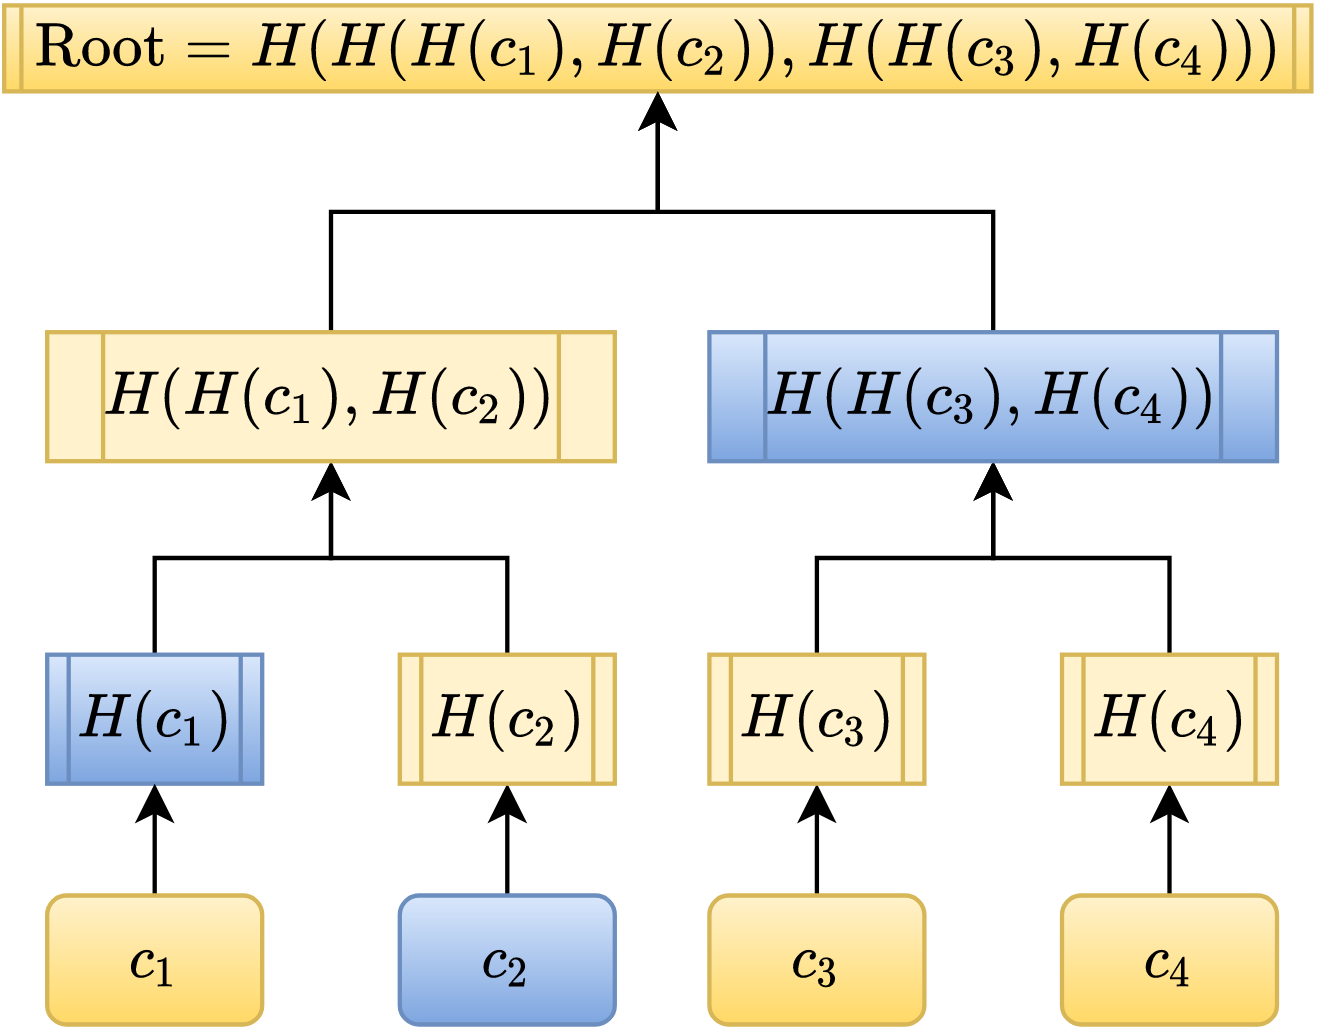
\includegraphics[width=0.4\textwidth]{image/merkletree.png}
    \definecolor{myColor1}{HTML}{7EA6E0}
    \caption{Merkle Tree example. \textbf{\textcolor{myColor1}{$c_2$'s siblings}}}
    \label{fig:merkletree}
\end{figure}
\begin{figure}[ht]
    \centering
    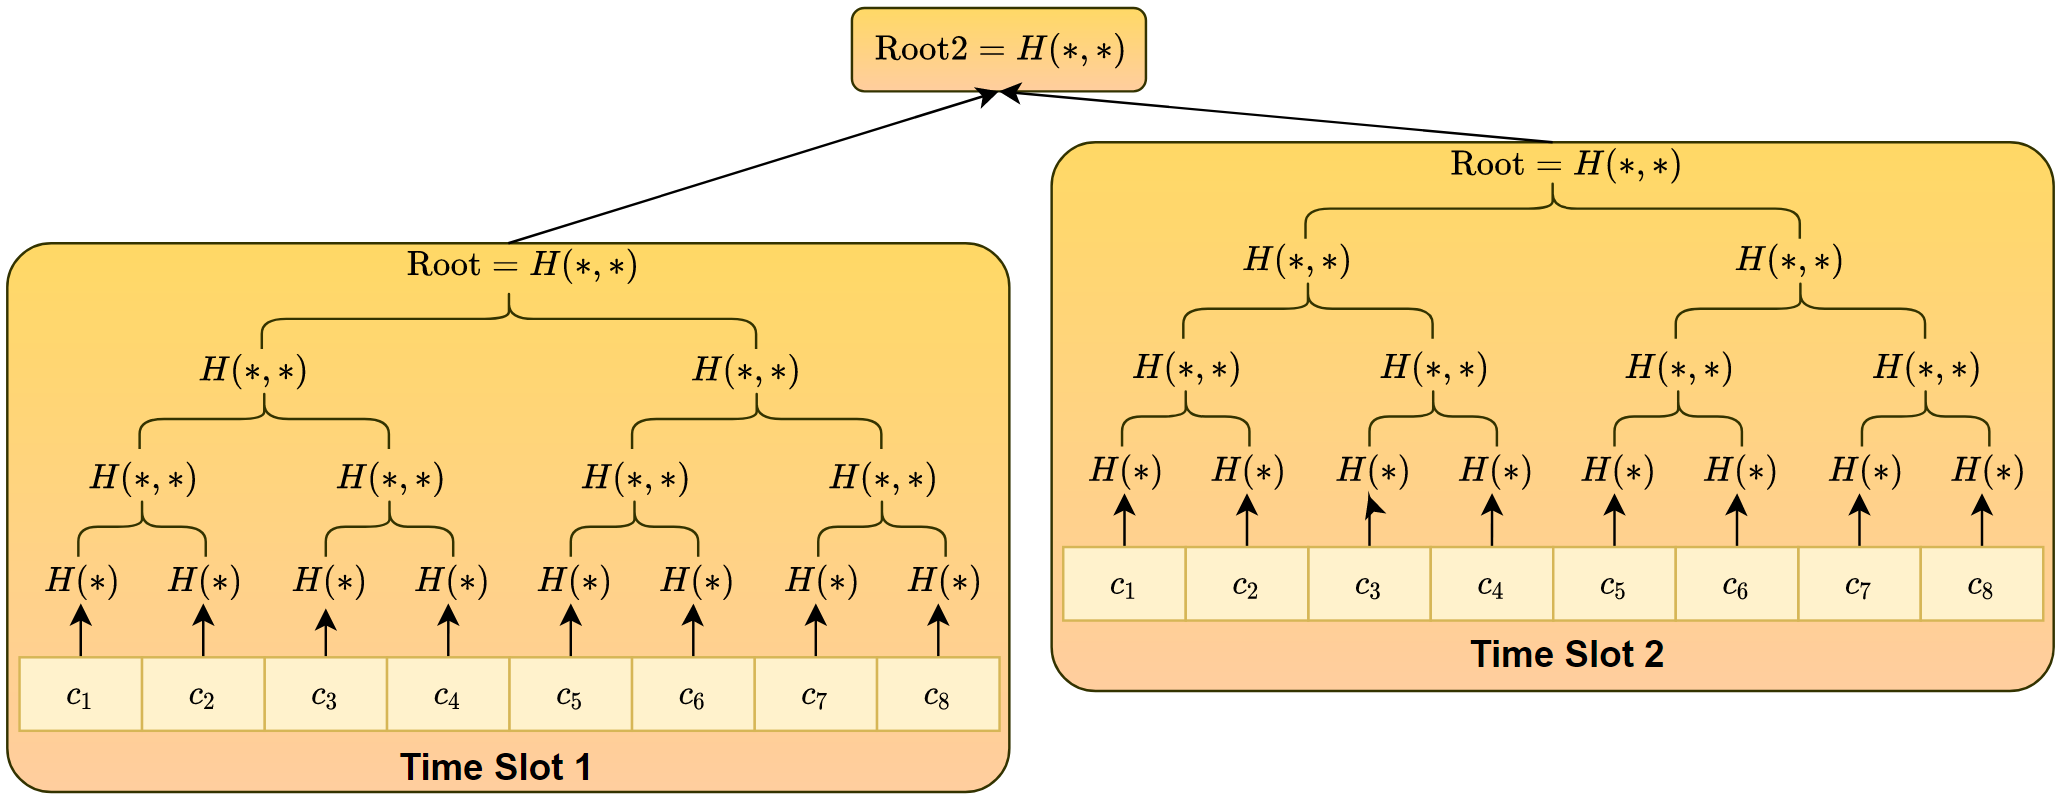
\includegraphics[width=0.9\textwidth]{image/merkletime.png}
    \caption{Merkle Tree with Time}
    \label{fig:merkletime}
\end{figure}
E' immediato dedurre che per verificare l'integrità di un chunk con un albero esteso servono:
\begin{proposition}[Integrity check wiht Time Extension]
\begin{itemize}
    \item I siblings dell'albero a cui appartiene il chunk.
    \item La radice dello slot temporale precedente.
    \item Le radici di tutti gli slot temporali successivi.
\end{itemize}
\end{proposition}
\begin{remark}
E' interessante notare come i merkle tree estesi permettano di costruire un sistema di \textbf{blockchain} per la verifica di certificati.
\end{remark}
\subsection{Certificate Transparency}
Il \textbf{processo} descritto nella \cref{def:certchain} è \textbf{debole} ad attacchi, perché \textbf{se un nodo} della catena \textbf{contiene} un \textbf{certificato falso}, allora il \textbf{sistema di autenticazione} è stato \textbf{rotto} a prescindere. Inoltre, \textbf{bisogna assicurarsi} che \textbf{la CA nella nostra lista possa rilasciare certificati}, come detto in \cref{thm:basiccons}.\\
Il problema descritto precedentemente può essere formalizzato così:
\begin{definition}[Fake Certificates Problem]
Una \textbf{CA intermedia} può generare \textbf{certificati malevoli} visti però come \textbf{validi} dalle entità, \textbf{compromettendo} i \textbf{meccanismi} di \textbf{autenticazione} e \textbf{recupero} delle chiavi pubbliche nella PKI.
\end{definition}
La soluzione venne proposta da Google nel 2013 e costituisce una mitigazione del problema, perché in ogni caso c'è una debolezza intrinseca alla base dell'infrastruttura.
\begin{note}
Se una delle entità universalmente fidate (es. Governi) dovesse, per qualche motivo, generare certificati malevoli non potremmo accorgerci di niente.
\end{note}
L'idea è quella di creare un DB scalabile globalmente distribuito.\pagebreak
\begin{multicols}{2}
\begin{definition}[CTDB]
Le caratteristiche del CTDB sono:
\begin{itemize}
    \item E' \textbf{globale, scalabile e sicuro} (non modificabile a posteriori).
    \item Può essere \textbf{amministrato} da \textbf{diversi stakeholders}.
    \item Tutte le CA possono inserire nel CTDB i certificati da loro emessi.
    \item Tutte le entità e le CA possono accedere e consultare il CTDB.
\end{itemize}
\end{definition}

\columnbreak
\begin{figure}[H]
    \centering
    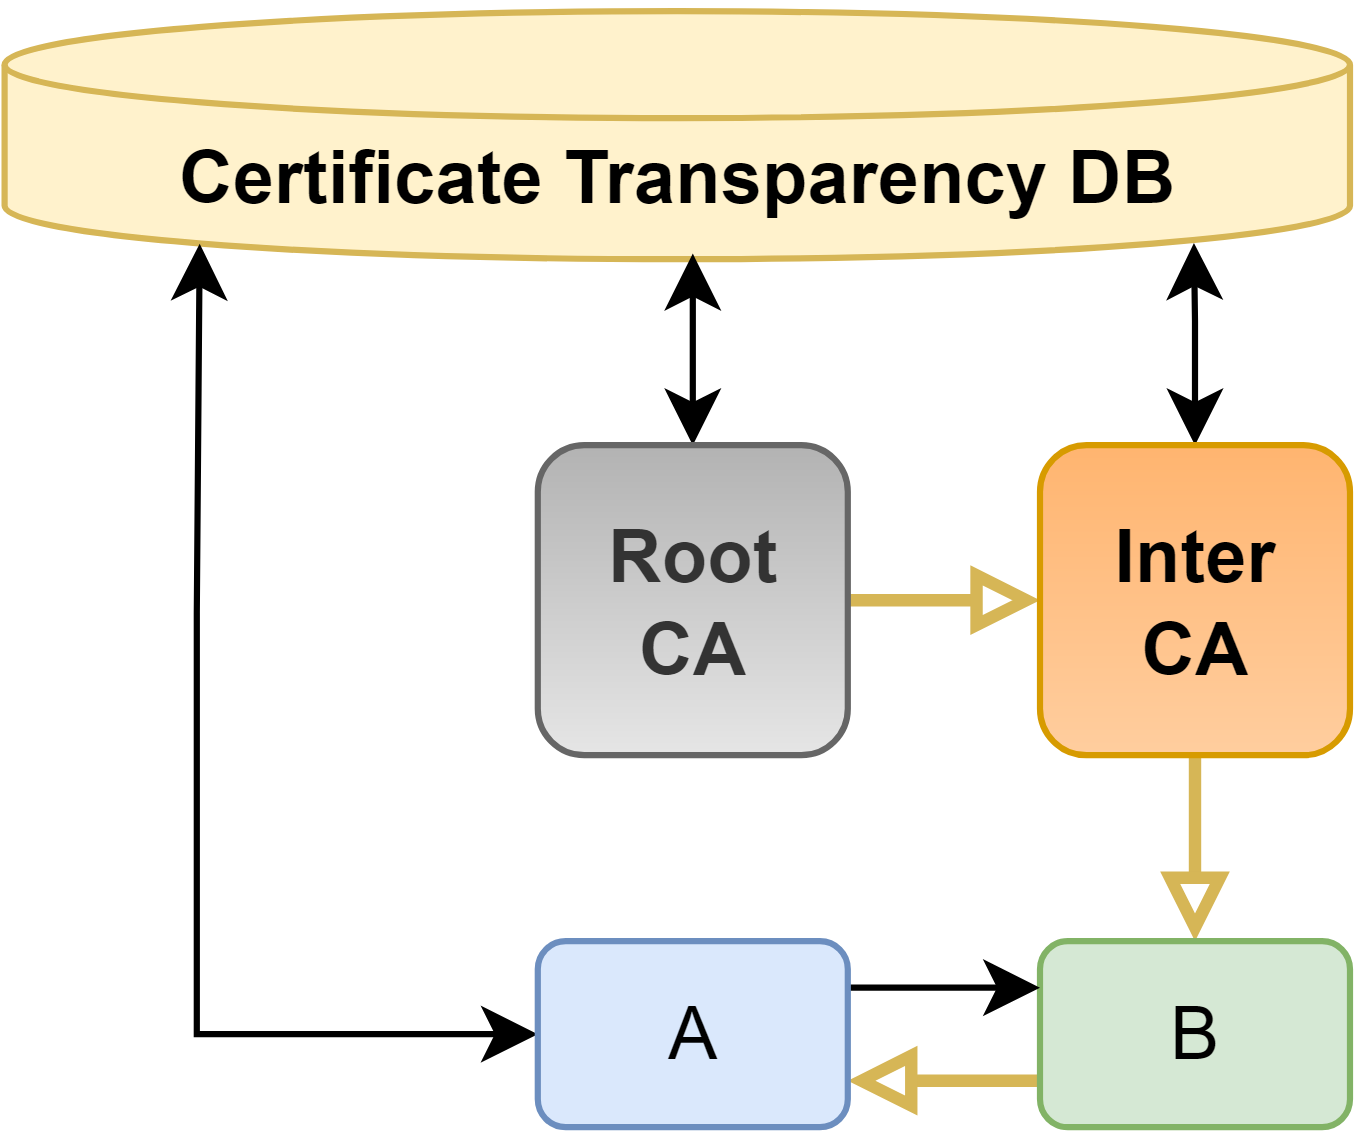
\includegraphics[width=0.4\textwidth]{image/certtrans.png}
    \caption{Certificate Transparency DB}
    \label{fig:certrans}
\end{figure}
\end{multicols}

Per soddisfare i requisiti funzionali il database è mantenuto in un \textbf{log server} (\textbf{unico e globalmente accessibile}), protetto
con uno schema derivante dai \textbf{Merkle's Tree esteso}, detto \textbf{Chron Tree}, caratterizzato dalle seguenti proprietà:
\begin{proposition}[Chron Tree Properties]
\begin{itemize}
    \item \textbf{Ogni certificato corrisponde ad un chunk}. Inoltre, ad ognuno di questi è aggiunto un \textbf{timestamp} per \textbf{evitare} l'\textbf{inserimento retroattivo} di certificati
    \item \textbf{L'albero è di tipo Append Only:} l'albero viene \textbf{esteso} ogni \textbf{24 ore} con un sottoalbero per la verifica della firma di tutti i certificati emessi dall'ultima estensione.
    \item \textbf{Consistency Proof:} ogni versione \textbf{successiva} del Merkle Tree \textbf{contiene per intero} la precedente come sottoalbero. Ciò rende \textbf{impossibile} la modifica di un certificato passato o l'inserimento di un \textbf{certificato retrodatato}.
    \item La verifica per un certificato necessita solamente del certificato stesso e dei siblings-tag all'interno dell'albero.
\end{itemize}
\end{proposition}
Le entità in gioco nel sistema descritto da \cref{fig:certrans} possono eseguire le seguenti operazioni:
\begin{proposition}[What a Requesting Entity can do]
Prima di utilizzare il certificato di un'entità B, l'entità richiedente A effettua i seguenti controlli:
\begin{enumerate}
    \item \textbf{Controlla} se il certificato digitale è \textbf{affidabile} tramite \textbf{certificate chain} e se è \textbf{valido}.
    \item\textbf{ Autentica B con un meccanismo CHAP-like}: A sottopone a B una \textbf{prova per la verifica della conoscenza la chiave privata} legata alla\textbf{ chiave pubblica nel certificato}.
    \item \textbf{Verifica che il certificato sia presente nel CTDB}: ricostruisce il tag root del sottoalbero del Merkle Tree esteso alla quale appartiene il certificato usando i siblings contenuti nel SCT (ricevuto insieme al certificato) e verifica la congruenza con quello presente nel log server.
    \item \textbf{Verifica che il certificato non sia presente in nessuna CRL delle CAs coinvolte.}
\end{enumerate}
\end{proposition}\pagebreak

\begin{proposition}[What a CA can do]
\begin{itemize}
    \item \textbf{Emettere un Certificato e Caricarlo nel CTDB}. In particolare vengono eseguite le seguenti operazioni:
    \begin{enumerate}
        \item La CA genera un \textbf{precertificato} temporaneo che invia al log-server.
        \item Il \textbf{log-server genera}, a partire dal precertificato, il relativo \textbf{certificato definitivo} e lo invia alla CA, \textbf{isieme} ad un \textbf{SCT (Signed Certificate Timestamp)}\footnotemark.
        \item La CA riceve la coppia \textbf{\{certificato, SCT\}} e la inoltra all'entità per la quale è stata generata. Per robustezza, sia CA che l'entità \textbf{mantengono localmente} il certificato e l'SCT.
        \footnotetext{\textsuperscript{\thefootnote}l'SCT contiene info aggiuntive necessarie alla verifica della validità del certificato, tra cui i siblings del sottoalbero a cui appartiene.}
    \end{enumerate}
    \item \textbf{Consultare il CRDB\footnotemark} alla ricerca di certificati malevoli emessi a suo nome, così da \textbf{inserirli} nella sua \textbf{CRL} ed ottenerne la revocazione.
    \footnotetext{\textsuperscript{\thefootnote}Certificate Revocation DB}
\end{itemize}
\end{proposition}

Il sistema di certificate transparency non è completamente primo di vulnerabilità. In particolare una CA intermedi corrotta a favore di un'entità B (non richiedente) potrebbe:
\begin{itemize}
    \item \textbf{Non aggiungere il certificato falso nel CTDB.} Tuttavia, l’entità A nota che il certificato per B non è presente del CTDB, e lo scarta a priori. \textbf{ L’attacco è perciò completamente neutralizzato.}
\item \textbf{Aggiungere un certificato falso/rubato nel CTDB.} Tuttavia, la CA proprietaria dell’identità rubata si accorgerebe subito del certificato falso inserito nella CTDB e lo aggiunge alla propria CRL.\\
L’\textbf{attacco} è perciò \textbf{mitigato}, in quanto può \textbf{esistere una finestra temporale} in cui il \textbf{certificato falso è nella CTDB ma non nella CRL}.
\end{itemize}
\begin{note}
La ceritificate transparency è diversa da un sistema a blockchain, sebbene siano entrambe protette da merkle tree. La differenza sta nel fatto che nelle \textbf{blockchain} le \textbf{transazioni} (i chunk) sono \textbf{vere se appartengono alla blockchain}.\\
Anche se è vero che un certificato viene considerato \textbf{falso} \textbf{se non appartiene} al CTDB, questo \textbf{può} ancora \textbf{essere falso} in quanto potrebbe esser stato \textbf{revocato} da una CA ed \textbf{appartenere} ad una \textbf{CRL}.
\end{note}
\pagebreak
\section{Authentication with Asymmetric Crypto}
Nel contesto della \textbf{comunicazione} sicura \textbf{basata sulla crittografia asimmetrica} e i \textbf{certificati digitali}, un’\textbf{entità} \textbf{può autenticarsi} dimostrando di conoscere la \textbf{chiave privata associata alla chiave pubblica} dichiarata all'interno del suo certificato. Esistono 2 diversi approcci:
\begin{itemize}
    \item \textbf{Firma Digitale}: il sistema autenticato dimostra la conoscenza della chiave privata generando la firma digitale per una challenge composta sia da una nonce che da testo arbitrario.
    \item \textbf{Decriptazione}: Il sistema autenticato dimostra la conoscenza della chiave privata, decriptando una challenge composta sia da una nonce che da un testo arbirario. La decriptazione può avvenire in due modi:
    \begin{itemize}
        \item \textbf{Asimmetrica:} Il sistema autenticato invia solamente la challenge criptata asimmetricamente.
        \item \textbf{Simmetrica con chiave di Sessione:} l'autenticatore invia una chiave di sessione casuale, criptata asimmetricamente e la challenge criptata simmetricamente.
    \end{itemize}
\end{itemize}
\begin{figure}[h]
    \centering
    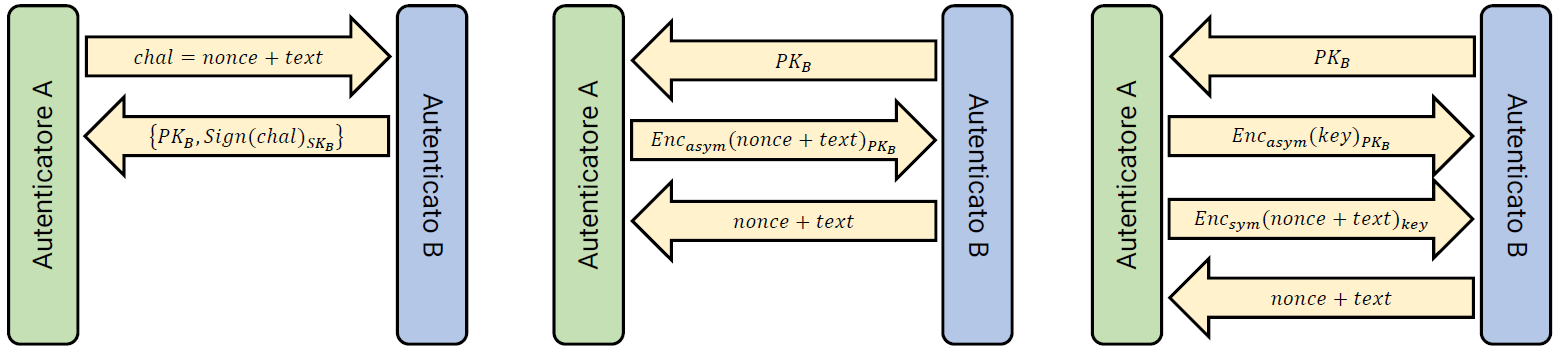
\includegraphics{image/authasymm.png}
    \caption{Authentication with Asymm Crypto}
    \label{fig:authasymm}
\end{figure}